\documentclass{article}

\usepackage[utf8]{inputenc}
\usepackage[T1]{fontenc}
\usepackage[frenchb]{babel}
\usepackage{tikz}
\usepackage{amsmath}
\usepackage{listings}
\usepackage{amssymb}
\usetikzlibrary{chains,positioning,matrix,arrows,decorations,calc}
\title{Rapport de projet : FMIN105\\ Cours algorithmique / complexité / calculabilité}
\author{\textsc{Bonavero} Yoann \\ \textsc{Brun} Bertrand \\ \textsc{Charron} John \\ \textsc{Dupéron} Georges}
\date{}

\setlength{\parindent}{0pt}
\setlength{\parskip}{2ex}

\newcounter{exocount}
\setcounter{exocount}{0}

\newcounter{enoncecount}
\setcounter{enoncecount}{0}

\newenvironment{enonce}
{
\stepcounter{enoncecount}
\bf\small \arabic{enoncecount}.
\begin{bf}
}
{
\end{bf}
}


\newcounter{sousenoncecount}
\setcounter{sousenoncecount}{0}
\newenvironment{sousenonce}
{
\stepcounter{sousenoncecount}
\bf\small (\alph{sousenoncecount})
\begin{bf}
}
{
\end{bf}
}

\begin{document}
\setcounter{page}{0}
\maketitle
\pagestyle{empty}
\thispagestyle{empty}
\tableofcontents
\pagestyle{empty}
\thispagestyle{empty}
\newpage
\pagestyle{plain}


\section{Descriptif des tâches}
Vos résultats seront présentés en procédant à la rédaction d'un mémoire dont la qualité influencera la note finale. Ce manuscrit sera rendu le jour de la soutenance. La soutenance consiste à présenter résultats pratiques (choix du langage, choix des structures de données, résultats obtenus, tests sur un grand jeu de données, analyse de ceux-ci ...) Vous aurez 15 minutes au maximum, questions comprises. Vous avez la possibilité d'utiliser des transparents.


\section{Partie théorique}
\subsection{Partie algorithmique}

\subsubsection*{Exercice \stepcounter{exocount}\bf\small \arabic{exocount} -- Modélisation et résolution d'un problème d'ordonnancement par un problème de flot maximum : ordonnancement avec coûts dépendants des dates de début}
\addcontentsline{toc}{subsubsection}{Exercice \arabic{exocount} -- Modélisation et résolution d'un problème d'ordonnancement par un problème de flot maximum : ordonnancement avec coûts dépendants des dates de début}



\begin{figure}[h!]
  \centering
  \begin{tikzpicture}[node distance=3cm]
    \node (J1) {$J_{1}$};
    \node (J2) [above of=J1] {$J_{2}$};
    \node (J3) [right of=J1] {$J_{3}$};
    \draw[->] (J1) -- (J2);
    \draw[->] (J1) -- (J3);
    \draw[->] (J3) -- (J2);
  \end{tikzpicture}
  \caption{Graphe G}
  \label{fig:graphe-g}
\end{figure}

\begin{enonce}
Construire le graphe $G*$ pour $n = 3$, $T = 5$, $p_1 = 1$, $p_2 = 2$, $p_3 = 1$, 
$E = \{(1,2), (1,3), (3,2)\}$ et les coûts suivants :
\end{enonce}

\begin{figure}[h!]
  \centering
	\begin{tabular}{cccccc}
	\hline	
	$i,t$ & 0 & 1 & 2 & 3 & 4\\
	\hline
	1 & 0 & 2 & 5 & 0 & 1\\
	2 & 1 & 1 & 2 & 4 & -\\
	3 & 1 & 10 & 2 & 3 & 3\\
	\hline
\end{tabular}
\end{figure}

\begin{figure}[h!]
  \centering
  \colorlet{affectation}{green!75!black}
  \colorlet{auxiliaire}{black}
  \colorlet{précédence}{blue}
  \begin{tikzpicture}[
      affectation/.style = {
        draw=affectation,
        ->
      },
      auxiliaire/.style = {
        draw=auxiliaire,
        ->
      },
      précédence/.style = {
        draw=précédence,
        ->
      },
      capacité/.style = {
        fill=white,
        font=\footnotesize
      },
      capacité affectation/.style = {
        text=affectation,
        capacité
      },
      capacité auxiliaire/.style = {
        text=auxiliaire,
        capacité
      },
      capacité précédence/.style = {
        text=précédence,
        capacité
      }
    ]
    
    \matrix[matrix of math nodes, nodes in empty cells, row sep=1cm, column sep=1cm] (m) {
      & v_{1,0} & v_{1,1} & v_{1,2} & v_{1,3} & v_{1,4} & v_{1,5} & \\
      s & v_{3,0} & v_{3,1} & v_{3,2} & v_{3,3} & v_{3,4} & v_{3,5} & t \\
      & v_{2,0} & v_{2,1} & v_{2,2} & v_{2,3} & v_{2,4} & & \\
    };
    
    %% Penser a rajouter les J1, J2 et J3 a gauche du graphe.
    
  	\draw[affectation] (m-1-2)-- node[capacité affectation]{0} (m-1-3);
	\draw[affectation] (m-1-3)-- node[capacité affectation]{2} (m-1-4);
	\draw[affectation] (m-1-4)-- node[capacité affectation]{5} (m-1-5);
	\draw[affectation] (m-1-5)-- node[capacité affectation]{0} (m-1-6);
	\draw[affectation] (m-1-6)-- node[capacité affectation]{1} (m-1-7);

	\draw[affectation] (m-2-2)-- node[capacité affectation]{1} (m-2-3);
	\draw[affectation] (m-2-3)-- node[capacité affectation]{10} (m-2-4);
	\draw[affectation] (m-2-4)-- node[capacité affectation]{2} (m-2-5);
	\draw[affectation] (m-2-5)-- node[capacité affectation]{3} (m-2-6);
	\draw[affectation] (m-2-6)-- node[capacité affectation]{3} (m-2-7);

	\draw[affectation] (m-3-2)-- node[capacité affectation]{1} (m-3-3);
	\draw[affectation] (m-3-3)-- node[capacité affectation]{1} (m-3-4);
	\draw[affectation] (m-3-4)-- node[capacité affectation]{2} (m-3-5);
	\draw[affectation] (m-3-5)-- node[capacité affectation]{4} (m-3-6);
	
  	\draw[auxiliaire] (m-2-1)-- node[capacité auxiliaire]{$\infty$} (m-1-2);
  	\draw[auxiliaire] (m-2-1)-- node[capacité auxiliaire]{$\infty$} (m-2-2);
  	\draw[auxiliaire] (m-2-1)-- node[capacité auxiliaire]{$\infty$} (m-3-2);
  	\draw[auxiliaire] (m-1-7)-- node[capacité auxiliaire]{$\infty$} (m-2-8);
  	\draw[auxiliaire] (m-2-7)-- node[capacité auxiliaire]{$\infty$} (m-2-8);
  	\draw[auxiliaire] (m-3-6)--(m-3-7.center)-- node[capacité auxiliaire]{$\infty$} (m-2-8);
	
	\draw[précédence] (m-1-2)-- node[capacité précédence]{$\infty$} (m-2-3);
	\draw[précédence] (m-1-3)-- node[capacité précédence]{$\infty$} (m-2-4);
	\draw[précédence] (m-1-4)-- node[capacité précédence]{$\infty$} (m-2-5);
	\draw[précédence] (m-1-5)-- node[capacité précédence]{$\infty$} (m-2-6);
	\draw[précédence] (m-1-6)-- node[capacité précédence]{$\infty$} (m-2-7);
    
	\draw[précédence] (m-2-2)-- node[capacité précédence]{$\infty$} (m-3-3);
	\draw[précédence] (m-2-3)-- node[capacité précédence]{$\infty$} (m-3-4);
	\draw[précédence] (m-2-4)-- node[capacité précédence]{$\infty$} (m-3-5);
	\draw[précédence] (m-2-5)-- node[capacité précédence]{$\infty$} (m-3-6);

	\draw[précédence] (m-1-2)-- node[capacité précédence,pos=0.3]{$\infty$} (m-3-3);
	\draw[précédence] (m-1-3)-- node[capacité précédence,pos=0.3]{$\infty$} (m-3-4);
	\draw[précédence] (m-1-4)-- node[capacité précédence,pos=0.3]{$\infty$} (m-3-5);
	\draw[précédence] (m-1-5)-- node[capacité précédence,pos=0.3]{$\infty$} (m-3-6);

  \end{tikzpicture}
  \caption{Graphe G*}
  \label{fig:graphe-g*}
\end{figure}



\begin{enonce}
Montrer qu'il existe une coupe dans G* de capacité minimale de laquelle sort un et un seul arc d'affectation par job.
\end{enonce}

Démonstration par construction~: 
On effectue un tri topologique sur le graphe des contraintes de précédence $G(\{J_1, \dots, J_n\}, E)$. Ce tri topologique nous donne un ensemble ordonné de n\oe uds $(J_{a1}, \dots, J_{an})$. On a donc~:
$$\forall J_{ai} \quad \nexists \ j < i \quad | \quad \exists (J_{aj}, J_{ai}) \in E$$
On transforme ensuite $G$ en un graphe de flots à l'aide de l'algorithme fourni dans le sujet. 
Considérons les arcs entre les $v_{ai,t}$~: 
\begin{itemize}
	\item Arcs d'affectation~: ces arcs sont entre des sommets $v_{ai,t}$ et $v_{aj,t'}$ avec $ai = aj$
	\item Arcs de précédences~: ces arcs sont entre des sommets $v_{ai,t}$ et $v_{aj,t'}$ avec $ai < aj$, car grâce au tri topologique, il n'existe pas d'arcs entre des sommets $J_{ai}$ et $J_{aj}$ avec $aj < ai$, et de plus il n'y a pas de boucle (donc pas d'arc $(J_{ai},J_{ai})$ dans $G$, donc pas d'arc $(v_{ai,t}, v_{ai,t'})$ dans $G*$).
	\item Arcs auxiliaires~: ces arcs ne sont pas entre des sommets $v_{ai,t}$.
\end{itemize}
On va créer une $(s-t)-\mathrm{coupe}$ minimale. Etant donné que cette coupe est minimale, aucun arc de capacité infinie n'a son origine dans $S$ et son extremité dans $\overline{S}$.

TODO~: Montrons que s'il s'agit d'une coupe minimale, il ne sort qu'un et qu'un
seul arc d'affectation par job. Il faut aussi montrer qu'il (il = ?) existe.

\begin{enonce}
Montrer que l'on peut associer un ordonnancement réalisable (qui respectent toutes les contraintes à toute 
coupe de capacité finie minimale dans le graphe. Quel est le coût de cet ordonnancement ? 
\end{enonce}

TODO~: Attention à la phrase suivante, ce n'est pas tout à fait ce qu'on a montré dans l'exercice 2

Dans l'exercice précédent, on a montré que de toute coupe minimale sort un et un seul arc d'affectation par job.

On cherche à associer un ordonancement réalisable à toute coupe minimale.

On va construire cet ordonancement de la manière suivante~: à chaque
fois qu'un arc d'affectation $v_{i,t}, v_{i,t+1}$ traverse la coupe,
on exécute le job $i$ à l'instant $t$ dans l'ordonancement.

On cherche un ordonancement, une suite de paires
$(\text{tâche},\text{date de début})$ respectant les dépendances. 
Autrement dit, chaque tâche apparaît après ses dépendances dans la
suite.

Comme chaque arc de précédence a une capacité finie, pour que la coupe
soit minimale, aucun arc de précédence ne doit sortir de la
coupe. Cela signifie qu'à chaque fois qu'on exécute un job (à
chaque fois qu'un arc d'affectation sort de la coupe), tous les arcs
de précédence entrants dans ce noeud ont leur extrémité déjà présente
dans la partie \og gauche \fg de la coupe 

TODO~: on n'a pas prouvé
cela, on l'a prouvé pour tous les arcs sortants, mais pas les arcs entrants. Il faut
montrer qu'en partant de la source, on est obligié d'avoir tous les
arcs de précédence entrants et donc que toutes les tâches dont dépend
celle-là (?) ont été exécutées à un temps antérieur (antérieurement ?).

On cherche un ordonancement réalisable, c'est-à-dire pour lequel
toutes les tâches peuvent être menées à bout durant le temps
imparti.

La propriété énoncée dans l'exercice 2 nous indique que dans toute
coupe minimale, un et un seul arc d'affectation par job sort de la
coupe. Cela signifie que chaque job a commencé à être exécuté. Comme
il exite un noeud pour le job $j$ à l'instant (à un instant donné ?) $t$ si et seulement s'il
y a le temps de l'exécuter (\ogà chaque date de début possible\fg),
cela signifie que tous les jobs commencés ont eu le temps d'être
terminés et, comme nous venons de voir, que tous les jobs ont pu être
commencés - ils ont tous pu être terminés - et, par conséquent, l'ordonancement est
réalisable.

\begin{enonce}
Montrer qu'à tout ordonnancement réalisable correspond une coupe dont la capacité est égale au coût de l'ordonnancement.
\end{enonce}

On construit la coupe à partir de l'ordonancement de la même manière
qu'on a construit l'ordonancement à partir de la coupe dans l'exercice
précédent, mais en suivant l'algorithme dans l'autre sens.

Si on exécute le job $i$ à l'instant $t$ dans l'ordonancement, alors
tous les noeuds $v_{i,t'}$ avec $t' \leq t$ sont dans la partie \og
gauche\fg de la coupe. De plus, (sujet de verba manquante ?) s'appartient lui aussi à la partie
gauche de la coupe.

TODO~: et les arcs de précédence ? Prouver qu'aucun ne sort de la
coupe dans notre construction.

La capacité de cette coupe est la somme de la capacité de tous les
arcs qui sortent de la coupe, c'est-à-dire la somme des capacités des
arcs $v_{i,t}, v_{i,t+1}$. Comme la capacité de ces arcs est égale au
coût d'exécution de la tâche $i$ à l'instant $t$, on a bien égalité entre
la somme des capacités et la somme des coûts de démarrage des jobs,
donc la capacité de la coupe est égale au coût de l'ordonancement.


\subsubsection*{Exercice \stepcounter{exocount}\bf\small \arabic{exocount} -- Coupes et chemins arc-disjoints}
\addcontentsline{toc}{subsubsection}{Exercice \arabic{exocount} -- Coupes et chemins arc-disjoints}
\setcounter{enoncecount}{0}

\begin{enonce}
Calculer le nombre maximum des chemins d'arcs disjoints à partir de la source jusqu'au puits dans le réseau donné par la figure 1. 
\end{enonce}

Il existe un ensemble de chemins d'arcs disjoints de cardinal 3~:

$$
\begin{array}{ccccccc}
  1 & \rightarrow & 2 & \rightarrow & 3 & \rightarrow & 6 \\
  1 & \rightarrow & 3 & \rightarrow & 4 & \rightarrow & 6 \\
  1 & \rightarrow & 4 & \rightarrow & 5 & \rightarrow & 6 \\
\end{array}
$$

Cherchons s'il en existe un de cardinal 4. Voici la liste des chemins
obtenue par un parcours en profondeur (en prennant toujours en premier
les sommets voisins avec le numéro le plus petit possible)~:

TODO~: numéroter les "équations"
$$
\begin{array}{ccccccccccc}
  1 & \rightarrow & 2 & \rightarrow & 3 & \rightarrow & 4 & \rightarrow & 5 & \rightarrow & 6 \\
  1 & \rightarrow & 2 & \rightarrow & 3 & \rightarrow & 4 & \rightarrow & 6 &             &   \\
  1 & \rightarrow & 2 & \rightarrow & 3 & \rightarrow & 6 &             &   &             &   \\
  1 & \rightarrow & 3 & \rightarrow & 4 & \rightarrow & 5 & \rightarrow & 6 &             &   \\
  1 & \rightarrow & 3 & \rightarrow & 4 & \rightarrow & 6 &             &   &             &   \\
  1 & \rightarrow & 3 & \rightarrow & 6 &             &   &             &   &             &   \\
  1 & \rightarrow & 4 & \rightarrow & 5 & \rightarrow & 6 &             &   &             &   \\
  1 & \rightarrow & 4 & \rightarrow & 6 &             &   &             &   &             &   \\
\end{array}
$$

Voyons les ensembles qui contiennent le chemin $A$~: On ne peut pas
prendre les chemins $B$ et $C$ car ils ont l'arc $(1,2)$ en commun
avec $A$. On ne peut pas prendre non plus les chemin $D$ et $G$ car
ils ont l'arc $(5,6)$ en commun avec $A$ ni le chemin $E$ à cause de
l'arc $(3,4)$. Il ne reste plus que les chemins $F$ et $H$ qu'on
pourrait peut-être prendre si on prend $A$, mais le cardinal de
l'ensemble serait alors 3, donc on n'améliorerait pas le résultat
existant. En conséquence, ce n'est pas la peine de chercher si ces chemins
sont \og compatibles\fg avec $A$.

Procédons de la même manière pour $B$ (sachant que $A$ ne peut pas
faire partie de l'ensemble). Si on a le chemin $B$, alors on ne peut
pas avoir~:
\begin{itemize}
  \item $C$ (arc $(2,3)$),
  \item $D$ (arc $(3,4)$),
  \item $E$ (arc $(3,4)$),
  \item $H$ (arc $(4,6)$).
\end{itemize}
À partir de ce moment, il ne reste plus que $F$ et $G$, l'ensemble
serait de cardinal 3, donc $B$ ne peut pas être dans un ensemble de
cardinal 4.

Passons à $D$ avec $A$ et $B$ exclus. On ne peut pas avoir~:
\begin{itemize}
\item $E$ (arc $(3,4)$),
\item $F$ (arc $(1,3)$),
\item $G$ (arc $(4,5)$).
\end{itemize}
Donc $D$ n'est pas dans l'ensemble.

Passons à $F$ avec $A,B,D$ exclus. On ne peut pas avoir~:
\begin{itemize}
\item $C$ (arc $(3,6)$),
\item $E$ (arc $(1,3)$).
\end{itemize}
Donc $F$ n'est pas dans l'ensemble.

Comme $A,B,D,F$ ne sont pas dans l'ensemble et que nous avons
seulement 8 candidats, la seule possibilité qui reste pour un ensemble
de cardinal 4 est $C,E,G,H$. Or, dans cet ensemble, l'arête $(1,4)$
est commune à $G$ et $H$, donc on ne peut pas construire un ensemble
de chemins d'arcs disjoints de taille 4 (donc pas de taille supérieure
à 4 non plus).

Conclusion~: Le nombre maximum de chemins d'arcs disjoints est 3.

\begin{enonce}
Enumérer tous les s-t-coupes dans le réseau donnés par la figure 1. Pour chaque s-t-coupe $[S,\overline{S}]$, énumérer les sommets, les arcs avants et les arcs arrières.
\end{enonce}

% Code LISP pour générer le tableau ci-après :

% (defun S (n p)
%   (if p
%       (format t "         ~a  " n)
%       (format t "\\phantom{~a} " n)))

% (defun Sbar (n p)
%   (S-n-p n (not p)))

% (defun print-arcs (arcs)
%   (when arcs
%     (when (car arcs)
%       (format t "(~a,~a)" (caar arcs) (cdar arcs))
%       (unless (endp (cdr arcs))
%         (format t ", ")))
%     (print-arcs (cdr arcs))))

% (defun print-arcs-if-not-nil (arcs)
%   (print-arcs (remove-if-not #'identity arcs)))

% (defun print-line (l nodes edges)
%   (let ((num-and-pred (pairlis nodes (mapcar #'list l))))
%     ;; (cdr (butlast)) pour ne pas imprimer les 1ers et derniers qui sont fixes.
%     (format t "~a " (car nodes))
%     (mapcar #'S (cdr (butlast nodes)) (cdr (butlast l)))
%     (format t "& ")
%     (mapcar #'Sbar (cdr (butlast nodes)) (cdr (butlast l)))
%     (format t "~a " (car (last nodes)))
%     (format t "& ${")
%     (print-arcs-if-not-nil
%      (mapcar (lambda (arc)
%                (and (cadr (assoc (car arc) num-and-pred))
%                     (not (cadr (assoc (cdr arc) num-and-pred)))
%                     arc))
%              edges))
%     (format t "}$ & ${")
%     (print-arcs-if-not-nil
%      (mapcar (lambda (arc)
%                (and (cadr (assoc (cdr arc) num-and-pred))
%                     (not (cadr (assoc (car arc) num-and-pred)))
%                     arc))
%              edges))
%     (format t "}$ \\\\~%")))

% (defun range (n)
%   (loop for i from 0 below n collect i))

% (defun print-s-t-cuts (nodes edges)
%   (loop
%      for i from 0 below (expt 2 (- (length nodes) 2))
%      do (print-line (append
%                      '(t) ;; Source : toujours t
%                      (mapcar (lambda (n)
%                                (/= 0 (logand i (expt 2 n))))
%                              (range (- (length nodes) 2)))
%                      '(nil)) ;; Target : toujours nil
%                     nodes
%                     edges)))

% (print-s-t-cuts
%  '(1 2 3 4 5 6)
% '((1 . 2)
%   (1 . 3)
%   (1 . 4)
%   (2 . 3)
%   (3 . 4)
%   (3 . 6)
%   (4 . 5)
%   (4 . 6)
%   (5 . 6)))

\begin{tabular}{|l|l|l|l|}
  \hline
  $S$ & $\overline{S}$ & Arcs avants & Arcs arrières \\
  \hline
  \hline
  1 \phantom{2} \phantom{3} \phantom{4} \phantom{5} &          2           3           4           5  6 & ${(1,2), (1,3), (1,4)}$               & ${}$             \\
  1          2  \phantom{3} \phantom{4} \phantom{5} & \phantom{2}          3           4           5  6 & ${(1,3), (1,4), (2,3)}$               & ${}$             \\
  1 \phantom{2}          3  \phantom{4} \phantom{5} &          2  \phantom{3}          4           5  6 & ${(1,2), (1,4), (3,4), (3,6)}$        & ${(2,3)}$        \\
  1          2           3  \phantom{4} \phantom{5} & \phantom{2} \phantom{3}          4           5  6 & ${(1,4), (3,4), (3,6)}$               & ${}$             \\
  1 \phantom{2} \phantom{3}          4  \phantom{5} &          2           3  \phantom{4}          5  6 & ${(1,2), (1,3), (4,5), (4,6)}$        & ${(3,4)}$        \\
  1          2  \phantom{3}          4  \phantom{5} & \phantom{2}          3  \phantom{4}          5  6 & ${(1,3), (2,3), (4,5), (4,6)}$        & ${(3,4)}$        \\
  1 \phantom{2}          3           4  \phantom{5} &          2  \phantom{3} \phantom{4}          5  6 & ${(1,2), (3,6), (4,5), (4,6)}$        & ${(2,3)}$        \\
  1          2           3           4  \phantom{5} & \phantom{2} \phantom{3} \phantom{4}          5  6 & ${(3,6), (4,5), (4,6)}$               & ${}$             \\
  1 \phantom{2} \phantom{3} \phantom{4}          5  &          2           3           4  \phantom{5} 6 & ${(1,2), (1,3), (1,4), (5,6)}$        & ${(4,5)}$        \\
  1          2  \phantom{3} \phantom{4}          5  & \phantom{2}          3           4  \phantom{5} 6 & ${(1,3), (1,4), (2,3), (5,6)}$        & ${(4,5)}$        \\
  1 \phantom{2}          3  \phantom{4}          5  &          2  \phantom{3}          4  \phantom{5} 6 & ${(1,2), (1,4), (3,4), (3,6), (5,6)}$ & ${(2,3), (4,5)}$ \\
  1          2           3  \phantom{4}          5  & \phantom{2} \phantom{3}          4  \phantom{5} 6 & ${(1,4), (3,4), (3,6), (5,6)}$        & ${(4,5)}$        \\
  1 \phantom{2} \phantom{3}          4           5  &          2           3  \phantom{4} \phantom{5} 6 & ${(1,2), (1,3), (4,6), (5,6)}$        & ${(3,4)}$        \\
  1          2  \phantom{3}          4           5  & \phantom{2}          3  \phantom{4} \phantom{5} 6 & ${(1,3), (2,3), (4,6), (5,6)}$        & ${(3,4)}$        \\
  1 \phantom{2}          3           4           5  &          2  \phantom{3} \phantom{4} \phantom{5} 6 & ${(1,2), (3,6), (4,6), (5,6)}$        & ${(2,3)}$        \\
  1          2           3           4           5  & \phantom{2} \phantom{3} \phantom{4} \phantom{5} 6 & ${(3,6), (4,6), (5,6)}$               & ${}$             \\
  \hline
\end{tabular}

\begin{enonce}
Vérifier que le nombre maximum de chemeins d'arcs disjoints à partir du sommet source jusqu'au puits est égal au nombre minimum d'arcs avant dans une s-t-coupe.
\end{enonce}

%% TODO

\subsection{Partie complexité}

\subsubsection*{Exercice \stepcounter{exocount}\bf\small \arabic{exocount} -- Sur quelques réductions}
\addcontentsline{toc}{subsubsection}{Exercice \arabic{exocount} -- Sur quelques réductions}
\setcounter{enoncecount}{0}

\begin{enonce}
On vous demande de rappeler la réduction de SAT à 3-SAT.
\end{enonce}

\begin{sousenonce}
Enoncer SAT et 3-SAT.
\end{sousenonce}

SAT est une abbrévation pour 'problème de satisfiabilité'. En logique propositionnelle, résoudre un problème SAT consiste à déterminer s'il existe une assignation des variables booléennes telle qu'une formule logique sous forme normale conjonctive s'évalue à vrai. Si tel est le cas, la formule est dite 'satisfiable', sinon elle est 'insatisfiable'. Etant donné le résultat booléen ('satisfiable' ou 'insatisfiable') de ce genre de problème, il s'agit bien d'un problème de décision.  

On appelle 2-sat un problème dont chaque clause de la formule logique en question contient au plus 2 littéraux, 3-sat un problème SAT dans lequel chaque clause de la formule logique en question contient au plus 3 littéraux. Un problème 2-sat est polynomial et NL-complet alors qu'un problème 3-sat est NP-complet.

Un exemple d'un problème 3-SAT est le suivant :

$(v_{1} \vee v_{2} \vee v_{3}) \wedge (v_{4} \vee v_{5} \vee v_{6}) \wedge (v_{7} \vee v_{8} \vee v_{9}) \wedge$ ...	

où chaque v est une variable ou la négation d'une variable, chaque variable pouvant figurer plusieurs fois dans l'expression. 

\begin{sousenonce}
Définir la réduction.
\end{sousenonce}

En théorie de complexité, une 'réduction' est la transformation d'un problème en un autre problème. Selon la transformation utilisée, la réduction peut être utilisée afin de définir une classe de complexité à un ensemble de problèmes. Problème A est réductible à Problème B si les solutions au Problème B existent et donnent des solutions au Problème A à chaque fois que A a des solutions. Par conséquent, la solution de A ne peut pas être plus difficile que la solution de B. 

Il peut être utile de résoudre un problème qui est similaire à un problème que l'on a déjà résolu. Dans ce cas, une méthode efficace de résoudre le nouveau problème est de transformer chaque instance du nouveau problème en une instance d'un problème que l'on sait résoudre et puis de résoudre chaque instance à l'aide de solutions existantes afin d'obtenir une solution finale. Une autre stratégie est de subdiviser un problème en plusieurs sous-problèmes que l'on sait résoudre, d'où le terme 'réduction'.

Une autre application des 'réductions' est son application aux problèmes qui sont difficiles à résoudre. Lorsque l'on a un problème qui a été prouvé difficile à résoudre et que nous avons un nouveau problème similaire, nous pouvons faire l'hypothèse que le nouveau problème, lui aussi, est difficile à résoudre. Le raisonnement est l'inverse de celui des problèmes qui peuvent être résolu aisément. 

Un exemple simple est de passer de la multiplication à la quadrature. Supposons que nous ne sommes capable que d'effectuer l'addition, la soustraction la quadrature et la division. Avec ces quatre opérations, nous pouvons trouver le produit de deux nombres quelconques :


$$(a \times b) = \dfrac{(a + b)^2 - a^2 - b^2}{2}$$


Lorsqu'il est possible de réduire un problème difficile en un problème que l'on sait résoudre, la difficulté demeure souvent dans la réduction elle-même.

GEORGES : Définition de la réduction de SAT à 3-SAT :

Pour la réduction de SAT à 3-SAT, on prend chaque clause de littéraux du problème SAT et on la transforme en une ou plusieurs clauses de la manière suivante~:

\begin{itemize}
\item Si la clause possède 3 littéraux ou moins, on la laisse telle quelle. Elle est déjà sous forme 3-SAT.
\item Sinon, soient $l_1, \dots, l_n$ les littéraux de la clause, on construit plusieurs clauses ainsi~:
$$
{l_1, l_2, z_1}, {\lnot z_1, l_3, z_2}, {\lnot z_2, l_4, z_3}, \dots, {\lnot z_{i-2}, l_{i}, z_{i-1}}, \dots, {\lnot z_{n-3}, l_{n-1}, l_{n}}
$$
\end{itemize}

Les littéraux $z_i$, qui n'était pas présents dans la clause d'origine, sont ajoutés afin de pouvoir subdiviser une clause en deux ou plusieurs les clauses et afin de les relier. Par exemple, la clause $(a \vee \lnot b \vee c \vee d)$ sera transformée en deux clauses~: $(a \vee \lnot b \vee z_1) \wedge (\lnot z_1 \vee c \vee d)$ ; la clause
${\lnot a \vee b \vee \lnot c \vee d \vee e}$ sera transformée en trois clauses, à savoir $(\lnot a \vee b \vee z_1) \wedge (\lnot z_1 \vee \lnot c \vee z_2) \wedge (\lnot z_2 \vee d \vee e)$.

L'ensemble des clauses ainsi créées sont équivalentes aux clauses d'origines correspondante car, à chaque fois, soit un des littéraux d'origine vérifie la clause, et $z_i$ peut être faux, ce qui permet au $\lnot z_i$ de valider la clause suivante, de proche en proche, soit aucun des littéraux d'origine ne vérifie la clause, auquel cas, si on prend un $z_i$ faux, la clause est fausse, et si on prend un $z_i$ vrai, la clause suivante contiendra
$\lnot z_i$ qui sera faux, et le résultat dépendra des littéraux de la ou des clause(s) suivante(s). 

% TODO BERTRAND: éclaircir ça, c'est mal expliqué.

Si l'on souhaite que le résultat soit strictement 3-SAT (toutes les clauses contenant exactement 3 littéraux, on applique les transformations suivantes~:
\begin{itemize}
\item Les clauses qui contiennent un seul littéral, ${l_1}$, sont transformées en ${l_1, l_1, l_1}$.
\item Les clauses qui contiennent exactement deux littéraux, ${l_1, l_2}$ sont transformées en ${l_1, l_2, l_1}$.
\end{itemize}

Cette transformation est linéaire en complexité. En effet, on ne considère chaque littéral qu'une fois et on ajoute $n-3$ littéraux pour chaque clause. Il s'agit de complexité polynomiale.

\begin{sousenonce}
Justifier alors que 3-SAT est NP-complet (sachant que SAT est NP-complet).
\end{sousenonce}

Vu que SAT est np-complet et que 3-SAT sait faire ce que sait faire SAT, avec une transformation polynomiale, 3-SAT (y compris la transformation) est au moins aussi dur que SAT. La difficulté peut résiter(??) dans la transformation, 3-SAT ou les deux.(??)

Vu que la difficulté ne s'est pas cachée dans la transformation, qui est polynomiale alors que SAT est np-complet, 3-SAT est np-complet lui aussi.  

\begin{sousenonce}
Application : si un ensemble de clauses contient $n_v$ variables, $n_1$ clauses à un littéral, $n_2$ clauses à 2 littéraux, $n_3$ clauses à 3 littéraux, $n_4$ clauses à 4 littéraux, $n_5$ clauses à 5 littéraux (et pas d'autres clauses), combien le système obtenu par votre réduction contient-il de variables et de clauses ? Vous devrez bien sûr justifier votre réponse.
\end{sousenonce}

Le système obtenu par la réduction contient :
\begin{itemize}
\item Une variable supplémentaire pour chaque clause à 4 littéraux.
\item Deux variables supplémentaires pour chaque clause à 5 littéraux.
\item Soit au total $n_v + n_4 + 2n_5$ variables.
\end{itemize}

De plus, les expansions sont les suivantes :
\begin{itemize}
\item Un littéral : 1 clause
\item Deux littéraux : 1 clause
\item Trois littéraux : 1 clause
\item Quatre littéraux : 2 clauses
\item Cinq littéraux : 3 clause
\item Soit au total $n_1 + n_2 + n_3 + 2n_4 + 3n_5$ clauses.
\end{itemize}


\begin{enonce}
Pourquoi le principe de la réduction ne permet-il pas de réduire 3-SAT à 2-SAT et de prouver que 2-SAT est NP-complet ? (Il ne s'agit pas d'expliquer pourquoi 2-SAT n'est pas NP-complet, mais pourquoi cette réduction ne marche pas).
\end{enonce}

Tentons de réduire la clause $(a \vee b \vee c)$ de manière similaire à l'algorithme donné pour la réduction de SAT à 3-SAT~. 

On a $(a \vee z_1) \wedge (\lnot z_1 \vee b)$. A partir de là, on ne peut insérer de variable permettant de faire la liaison entre la clause qui contient $b$ et celle qui contient $c$.

TODO: Cette question, est-elle répondue ? 

\begin{enonce}
Il s'agit de prouver que 2-SAT est un problème polynomial. Vous avez un article en français expliquant cette preuve à \\ http://philippe.gambette.free.fr/SCOL/Graphes
\end{enonce}
\setcounter{sousenoncecount}{0}

\begin{sousenonce}
Vous commencerez par fabriquer trois ensembles de deux clauses, le premier valide, le deuxième insatisfiable et le troisième contingent, et pour chacun de ces ensembles de clauses vous construirez le graphe correspondant. Vous expliquerez comment apparaît sur chacun des trois graphes la validité de l'ensemble de clauses corresponsdantes.
\end{sousenonce}

Philippe Gambette, dans son article intitulé 'Un graphe pour résoudre 2-SAT', donne une explication succincte de l'agorithme d'Aspvall, Plass et Tarjan.

Une formule logique en forme normale conjonctive contenant des clauses à deux littéraux est transformé en un problème de graphe orienté. On doit tout d'abord établir si la formule admet un modèle, et ensuite, si tel est le cas, donner un modèle quelconque.

\begin{enumerate}
\item L'algorithme du construction de graphe : 
\begin{enumerate}
\item On crée un graphe avec $2n$ sommets ($n$ étant ici le nombre littéraux distincts de la formule) contenant tous les littéraux de la formule ainsi que les négations de ces littéraux.
\item On prend chaque clause de la formule que l'on traduit en implications dans les deux sens : $(a \vee b)$ 
se transforme en deux clauses : $(\neg a \Rightarrow b)$ et ($\neg b \Rightarrow a)$.
\item On crée des arcs correspondant aux implications créées à l'étape précédente (arc ($\neg a 
\rightarrow b$) et ($\neg b \rightarrow a$))
\end{enumerate}
\item On effectue un tri topologique en numérotant les sommets de $1$ à $n$.
\item En ordre inverse, du sommet $n$ au sommet $1$ du graphe, on affecte à tout noeud $x$ la valeur VRAI et au noeud $\neg x$ la valeur FAUX, c'est-à-dire dans l'ordre inverse du tri topologique.
\end{enumerate}  	

S'il existe une composante fortement connexe contenant un littéral et sa négation, la formule est insatisfiable étant donné qu'on a $x_{i} \Leftrightarrow \neg £x_{i}$ sinon, la formule est satisfiable, c'est-à-dire soit contingente soit valide. L'algorithme ne nous donne aucune information pour distinguer une formule contingente et une formule valide, il nous donne une ou deux informations : (1) il nous dit si la formule admet un modèle, et (2) si oui, il nous donne un modèle~: le modèle est assuré car le graphe en question ne contient aucun arc $VRAI \rightarrow FAUX$.

Prenons trois exemples~: une formule insatisfiable, une formule contingente et une formule valide.

\begin{figure}[h!]
  \centering
  \begin{tikzpicture}[
      node distance=2.5cm,
      lettre/.style={
        draw,
        circle,
        minimum size=1cm
      }
    ]
    \node[lettre] (nx1) {$\lnot x_1$} ;
    \node[lettre, below of=nx1] (x1) {$x_1$} ;
    \node[coordinate,xshift=0.1cm] (x1r) at (x1.north) {};
    \node[coordinate,xshift=-0.1cm] (x1l) at (x1.north) {};
    \node[coordinate,xshift=0.1cm] (nx1r) at (nx1.south) {};
    \node[coordinate,xshift=-0.1cm] (nx1l) at (nx1.south) {};
    \draw[->] (x1r) -- (nx1r);
    \draw[->] (nx1l) -- (x1l);
    \path
      (x1) edge[loop below] (x1)
      (nx1) edge[loop above] (nx1) ;
  \end{tikzpicture}
  \caption{Clause insatisfiable : $(x_{1} \vee x_{1}) \wedge (\neg x_{1} \vee \neg x_{1})$}
  \label{fig:clause-insat}
\end{figure}

\paragraph*{Clause insatisfiable $(x_{1} \vee x_{1}) \wedge (\neg x_{1} \vee \neg x_{1})$~:}

Le résultat de l'application de l'algorithme décrit ci-dessus est un graphe orienté cyclique. Il est impossible d'effectuer un tri topologique étant donné qu'un tri topologique ne peut être effectué que sur un graphe acyclique orienté. Ce graphe contient un composant fortement connexe contenant un littéral et sa négation, et la formule associée est, par conséquent, insatisfiable. Il est impossible d'attribuer un ordre aux sommets pour ensuite affecter des valeurs aux littéraux correspondant aux sommets car la formule admet aucun modèle. Pour cette raison, les arcs de ce graphe n'ont pas été numérotés ni affectés des valeurs $VRAI$ ou $FAUX$. En somme, l'algorithme nous dit simplement que ce graphe n'admet aucun modèle.

\begin{figure}[h!]
  \centering
  \begin{tikzpicture}[
      start chain=circle placed {at=(\tikzchaincount*-45+22.5+90:2.5)},
      lettre/.style={
        on chain,
        draw,
        circle,
        minimum size=1cm
      },
      chiffre/.style={
        node distance = 0.75cm
      },
      arr/.style={
        ->,
        >=triangle 90
      }
    ]
    \node[lettre] (1) {$\lnot x1$} ;
    \node[lettre] (5) {$x2$} ;
    \node[lettre] (3) {$\lnot x2$} ;
    \node[lettre] (6) {$x3$} ;
    \node[lettre] (4) {$\lnot x3$} ;
    \node[lettre] (7) {$x4$} ;
    \node[lettre] (2) {$\lnot x4$} ;
    \node[lettre] (8) {$x1$} ;
    
    \node[right of=1] {\textcolor{red}{faux}} ;
    \node[right of=5] {\textcolor{green!75!black}{vrai}} ;
    \node[right of=3] {\textcolor{red}{faux}} ;
    \node[right of=6] {\textcolor{green!75!black}{vrai}} ;
    \node[left  of=4] {\textcolor{red}{faux}} ;
    \node[left  of=7] {\textcolor{green!75!black}{vrai}} ;
    \node[left  of=2] {\textcolor{red}{faux}} ;
    \node[left  of=8] {\textcolor{green!75!black}{vrai}} ;
    
    \node[chiffre, above right of=1] {1} ;
    \node[chiffre, above right of=5] {5} ;
    \node[chiffre, below right of=3] {3} ;
    \node[chiffre, below right of=6] {6} ;
    \node[chiffre, below left of=4]  {4} ;
    \node[chiffre, below left of=7]  {7} ;
    \node[chiffre, above left of=2]  {2} ;
    \node[chiffre, above left of=8]  {8} ;

    \draw[arr] (1) -- (5) ;
    \draw[arr] (3) -- (8) ;
    \draw[arr] (2) -- (6) ;
    \draw[arr] (4) -- (7) ;
  \end{tikzpicture}
  \caption{Clause contingente : $(x_{1} \vee x_{2}) \wedge (x_{3} \vee x_{4})$}
  \label{fig:clause-conting}
\end{figure}

% \includegraphics[height=2in, width = 3in]{img/contingente.png

\paragraph*{Clause contingente $(x_{1} \vee x_{2}) \wedge (x_{3} \vee x_{4})$~:}
Le graphe de la figure \ref{fig:clause-conting} ne contient aucune composante fortement connexe contenant un littéral et sa négation, donc la formule associée admet bien un modèle. Ce modèle est le résultat du tri topologique effectué et les valeurs $VRAI$ et $FAUX$ affectées à des sommets par notre algorithme. Il existe aucun arc qui part d'un sommet étiqueté $VRAI$ vers un sommet étiqueté $FAUX$ et, en effet, les valeurs attribuées aux arcs donnent bien un modèle. 



\begin{figure}[h!]
  \centering
  \begin{tikzpicture}[
      start chain=circle placed {at=(\tikzchaincount*-90+180:1.6)},
      lettre/.style={
        on chain,
        draw,
        circle,
        minimum size=1cm
      },
      chiffre/.style={
        node distance = 0.75cm
      },
      arr/.style={
        ->,
        >=triangle 90
      }
    ]
    \node[lettre] (1) {$\lnot x1$} ;
    \node[lettre] (2) {$x1$}  ;
    \node[lettre] (3) {$\lnot x2$} ;
    \node[lettre] (4) {$x2$}  ;
    
    \node[right of=1] {\textcolor{green!75!black}{vrai}} ;
    \node[right of=2] {\textcolor{red}{faux}} ;
    \node[right of=3] {\textcolor{green!75!black}{vrai}} ;
    \node[left  of=4] {\textcolor{red}{faux}} ;
    
    \node[chiffre, above right of=1] {1} ;
    \node[chiffre, below right of=2] {2} ;
    \node[chiffre, below right of=3]  {3} ;
    \node[chiffre, below left of=4]  {4} ;

	\path
       (1) edge[loop above] (1)
       (2) edge[loop above]  (2)
       (3) edge[loop below] (3)
       (4) edge[loop above] (4) ;
  \end{tikzpicture}
  \caption{Clause valide :  $(x_{1} \vee \neg x_{1}) \wedge (x_{2} \vee \neg x_{2})$}
  \label{fig:clause-valide}
\end{figure}

% 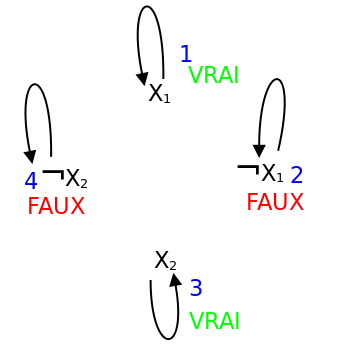
\includegraphics[height=2in, width = 3in]{img/valide.png}

\paragraph*{Clause valide $(x_{1} \vee \neg x_{1}) \wedge (x_{2} \vee \neg x_{2})$~:}
L'application de l'algorithme de transformation en graphe d'une formule valide nous donne un graphe ne contenant que des boucles à chaque sommet. Nous pouvons donc numéroter les arcs de n'importe quel façon. Ce étant, nous pouvous aussi affecter n'importe quelles valeurs aux sommets (hormis la même valeur à un littéral et sa négation, bien entendu) et la formule sera toujours vraie. 

L'objectif de cet algorithme n'est pas de dire si une formule satisfiable est contingente ou valide. Toutefois, si le résultat de l'algorithme est un graphe ne comportant que des boucles à chaque sommet, la formule associée est satisfiable et valide. Autrement, et si le graphe ne contient aucune composante fortement connexe contenant un littéral et sa négation, la formule est contingente.

TODO: VERIFIER CES DEUX DERNIERS PHRASES (PRECEDENTES), EST-CE QUE C'EST JUSTE ? C'EST MOI QUI A FAIT CES CONSTATATIONS 

\begin{sousenonce}
Vous expliciterez ensuite l'algorithme de transformation et vous évaluerez sa complexité.
\end{sousenonce}

TODO: GEORGES -> J'ai trouvé la citation du CORMEN que j'ai mis ici, mais je ne sais pas comment répondre à cette question avec justesse. Donc, j'ai trouvé toutes les infos, peut-être que quelqu'un pourrait finir cette question. On supprime, bien entendu, cette sitation de CORMEN. Merci, JC.
JE NE SUIS PAS DU TOUT SUR DE LA REPONSE A CETTE QUESTION... J'AI COMMENCE A REDIGER, MAIS...

Tout d'abord, il faut transformer une formule en forme normale conjonctive en une série d'implications. Cela se fait en temps linéaire, en $O(n)$. Ensuite, il faut créer le graphe associé -- numérotation et attribution des valeurs $VRAI$ et $FAUX$, ce qui se fait également en 0(n). 


CORMEN:
We can perform a topological sort in time , since depth-first search takes $\theta(V + E)$
time and it takes O(1) time to insert each of the |V| vertices onto the front of the linked list.


Our algorithm for finding strongly connected components of a graph G = (V, E) uses the
transpose of G, which is defined in Exercise 22.1-3 to be the graph GT = (V, ET), where ET =
{(u, v) : (v, u) E}. That is, ET consists of the edges of G with their directions reversed. Given
an adjacency-list representation of G, the time to create GT is O(V + E). It is interesting to
observe that G and GT have exactly the same strongly connected components: u and v are
reachable from each other in G if and only if they are reachable from each other in GT. Figure
22.9(b) shows the transpose of the graph in Figure 22.9(a), with the strongly connected
components shaded.
The following linear-time (i.e., $\theta(V + E)$-time) algorithm computes the strongly connected
components of a directed graph G = (V, E) using two depth-first searches, one on G and one
on GT.
STRONGLY-CONNECTED-COMPONENTS (G)
1 call DFS (G) to compute finishing times f[u] for each vertex u
2 compute GT
3 call DFS (GT), but in the main loop of DFS, consider the vertices
in order of decreasing f[u] (as computed in line 1)
4 output the vertices of each tree in the depth-first forest formed in
line 3 as a
separate strongly connected component

\begin{sousenonce}
Vous expliciterez ensuite l'algorithme d'exploration du graphe et vous évaluerez sa complexité
 en fonction de la taille de l'ensemble de clauses initial.
\end{sousenonce}

TODO: J'ai répondu en quelques lignes ci-dessous, mais je ne sais pas du tout si ce que j'ai dit est juste. Quelqu'un pourrait le compléter ou le refaire, cette partie ? Merci, JC.

Le tri topologique se fait en $\theta(V + E)$ en faisant un parcours en profondeur. Etablir s'il existe une composante connexe (sans prendre en compte, pour l'instant, si ce composant contient un sommet ainsi que sa négation) se fait en $O(V + E)$. Etablir s'il existe un littéral et sa négation se fait en temps linéaire $O(n)$. 

Tout l'algorithme se fait donc en temps linéaire, en $theta(V + E)$

\begin{sousenonce}
Enfin, vous justifierez l'équivalence de la réponse au problème 2-SAT et au problème qui est posé dans le graphe.
\end{sousenonce}

TODO: Désolé, mais je ne maîtrise pas du tout ... Help !! (JC)

\subsection{Partie Calculabilité}

\subsubsection*{Exercice \stepcounter{exocount}\bf\small \arabic{exocount} -- Sur le problème de codage}
\addcontentsline{toc}{subsubsection}{Exercice \arabic{exocount} -- Sur le problème de codage}
\setcounter{enoncecount}{0}

\begin{enonce}
Comment énumérer les couples d'entiers ?
\end{enonce}


L'énumération des couples de manière relativement homogène nous donnerait un codage qui nous permettrait d'identifier chaque couple par un nombre unique. 

Il ne serait pas du tout utile de commencer par tous les couples $(0,y_{i})$  tel que $i \in \mathbb{Z}$ car il s'agirait, là, d'un ensemble infini de couples et on ne passerait jamais aux couples $(1, y_{i})$. 

Une solution, pour tous les nombres naturels, serait de parcourir un graphe comme suit:

\begin{figure}[h!]
  \centering
  \begin{tikzpicture}[
      dot/.style = {
        circle,
        fill=black,
        inner sep=0.5pt
      },
      arc/.style = {
        ->,
        >=stealth
      }
    ]
    \foreach \xpos in {0, ..., 4} {
      \foreach \ypos in {0, ..., 4} {
        \node[dot] at (\xpos,-\ypos) {};
      }
    }
    
    \draw[arc] (0,-0) -- (1,-0);
    
    \draw[arc] (1,-0) -- (0,-1);
    \draw[arc] (0,-1) -- (0,-2);
    
    \draw[arc] (0,-2) -- (1,-1);
    \draw[arc] (1,-1) -- (2,-0);
    \draw[arc] (2,-0) -- (3,-0);
    
    \draw[arc] (3,-0) -- (2,-1);
    \draw[arc] (2,-1) -- (1,-2);
    \draw[arc] (1,-2) -- (0,-3);
    \draw[arc] (0,-3) -- (0,-4);
    
    \draw[arc] (0,-4) -- (1,-3);
    \draw[arc,dashed] (1,-3) -- (2,-2);
  \end{tikzpicture}
  \caption{Graphe G}
  \label{fig:codage-zigzag}
\end{figure}

TODO: Il faudrait ajouter les coordonnées (0,0), (1,0), (0,1), et les codes correspondants au graphe ci-dessus, etc. VOIR LES DIAGRAMMES QUE J'AI DONNE A BERTRAND

Dans la figure \ref{fig:codage-zigzag}, on commence par le couple $(0,0)$, puis on procède aux couples $(1,0)$, $(0,1)$, $(0,2)$, $(1,1)$, $(2,0)$, $(3,0)$, $(2,1)$, $(1,2)$, $(0,3)$, $(0,4)$\ldots L'algorithme pour simplement parcourir les couples de cette façon consisterait tout d'abord de déclarer et d'intialiser trois variables globales~: le point de départ, \lstinline!*current*!, et les valeurs maximales courantes de $x$ et de $y$, c'est-à-dire \lstinline!*max-x*! et \lstinline!*max-y*!. En LISP, ceci pourrait être codé comme suit~:

\begin{lstlisting}[language=Lisp]
(defvar *current* (list 0 0 0)) ;; liste courante (code x y)
(setf *current* (list 0 0 0)) 
(defvar *max-x* 0) ;; valeur maximal courante de x
(setf *max-x* 0)
(defvar *max-y* 0) ;; valeur maximal courante de y
(setf *max-y* 0)
\end{lstlisting}

On pourrait stocker toutes les valeurs de \lstinline!*current*! dans un tableau \lstinline!*db*! (base de données) comme suit~:

\begin{lstlisting}[language=Lisp]
(defvar *db* nil) 
(setf *db* nil)
(push *current* *db*)
\end{lstlisting}

Puis, les conditions pour déterminer la direction à prendre afin de parcourir le graphe pourrait être implémentées comme suit (toujours en LISP)~:

\begin{lstlisting}[language=Lisp]
(defun move (L)
  (cond
    ((and (zerop (third L)) (= *max-x* *max-y*)) 
		;; RIGHT takes precedence over LEFT becuase it occurs first
      (print "in RIGHT") ;; 
         (right L))
    ((and (zerop (second L)) (= *max-x* *max-y*)) ;; DOWN
      (print "in DOWN") 
         (down L))
    ((> *max-x* *max-y*) ;; DOWN-LEFT
      (print "in DOWN-LEFT")  
         (down-left L))
    ((< *max-x* *max-y*) ;; UP-RIGHT
      (print "in UP-RIGHT") 
         (up-right L))))
\end{lstlisting}
 
La liste \lstinline!*current*! est passée en paramètre lorsque l'on appelle ces fonctions~: L correspond toujours à *current*. Les fonctions 'right', 'down', 'down-left' et 'up-right', qui correspondent au parcours dans la figure ???, incrémente la première valeur de L (le codage), qui est une liste de la forme \lstinline!(code x y)!. Par ailleurs, la fonction 'right' incrémente la valeur courante de $x$ (le deuxième élément de la liste), la fonction 'down' incrémente la valeur courante de $y$ (la troisième élément de la liste), la fonction 'down-left' décrémente la valeur de $x$ et incrémente la valeur $y$ et la fonction 'up-right', elle, fait le contraire, elle incrémente la valeur de $x$ et décrémente la valeur de $y$. 

On peut parcourir le graphe à l'aide de la fonction 'zig-zag' qui, elle, se sert de la fonction move-and-update afin de mettre à jour les variables globales *max-x* et *max-y*. 'move-and-update' se sert de 'move' qui choisit la bonne direction à prendre pour parcourir le graphe, c'est-à-dire 'right', 'down', 'down-left' ou 'up-right'~:

\begin{lstlisting}[language=Lisp]
(defun move-and-update (L)
  (progn
    (setf L (move L))
    (update-max-x-y L)
    *db*))
 
(defun zig-zag (L n)
    (if (zerop n) 
      (move-and-update *current*)
      (progn
        (move-and-update *current*)
        (zig-zag L (- n 1)))))
\end{lstlisting}


%% TODO : JOHN :
%% Pour définir un label pour une section / sous-section / …, il faut mettre ceci juste après le \section{…}
%% \label{foobar}
%%
%% Pour avoir le numéro de page correspondant :
%% \pageref{foobar}
%%
%% Pour le numéro de section / sous-section / … :
%% \ref{foobar}
%%
%% Tu changes foobar par un nom de ton choix.
L'intégralité du programme est en annexe à la page ???. Il existe également une version en C à la page ??.

Voici une trace de cette fonction en passant \lstinline!*current*! égal à \lstinline!(0 0 0)! en paramètre et avec $n = 100$ :

\begin{lstlisting}[language=Lisp]
> (zig-zag *current* 100)
"in RIGHT" 
"in DOWN-LEFT" 
"in DOWN" 
"in UP-RIGHT" 
"in UP-RIGHT" 
"in RIGHT" 
(etc.)
"in DOWN-LEFT" 
"in DOWN-LEFT" 
((101 3 10) (100 4 9) (99 5 8) (98 6 7) (97 7 6) (96 8 5) 
(95 9 4) (94 10 3) (93 11 2) (92 12 1) (91 13 0) (90 12 0) 
(89 11 1) (88 10 2) (87 9 3) (86 8 4) (85 7 5) (84 6 6) 
(83 5 7) (82 4 8) (81 3 9) (80 2 10) (79 1 11) (78 0 12) 
(77 0 11) (76 1 10) (75 2 9) (74 3 8) (73 4 7) (72 5 6) 
(71 6 5) (70 7 4) (69 8 3) (68 9 2) (67 10 1) (66 11 0) 
(65 10 0) (64 9 1) (63 8 2) (62 7 3) (61 6 4) (60 5 5) 
(59 4 6) (58 3 7) (57 2 8) (56 1 9) (55 0 10) (54 0 9) 
(53 1 8) (52 2 7) (51 3 6) (50 4 5) (49 5 4) (48 6 3) 
(47 7 2) (46 8 1) (45 9 0) (44 8 0) (43 7 1) (42 6 2) 
(41 5 3) (40 4 4) (39 3 5) (38 2 6) (37 1 7) (36 0 8) 
(35 0 7) (34 1 6) (33 2 5) (32 3 4) (31 4 3) (30 5 2) 
(29 6 1) (28 7 0) (27 6 0) (26 5 1) (25 4 2) (24 3 3) 
(23 2 4) (22 1 5) (21 0 6) (20 0 5) (19 1 4) (18 2 3) 
(17 3 2) (16 4 1) (15 5 0) (14 4 0) (13 3 1) (12 2 2) 
(11 1 3) (10 0 4) (9 0 3) (8 1 2) (7 2 1) (6 3 0) (5 2 0) 
(4 1 1) (3 0 2) (2 0 1) (1 1 0) (0 0 0))
\end{lstlisting}


\begin{enonce}
Donner les fonctions de codage et de décodage f1(z)->x et f2(z)->y.
\end{enonce}

TODO: Même figure que la précédente, mais avec les 'constations' ajoutées (je ferai un diagramme papier pour qu'on sache ce que je veux ici)

En reprenant la figure ??? ci-dessus, on peut faire plusieurs constatations~:

\begin{itemize}
\item La somme de $x$ et $y$ de chaque sommet du graphe d'une diagonale dans le sens du parcours est toujours la même.
\item La longueur de chaque diagonale successive s'incrémente à chaque fois et nous donne par conséquent toujours une longueur impaire suivie d'une longueur paire.
\item Le point à partir duquel on commence à incrémenter le code au long d'une diagonale correspond aux codes $1$, $3$, $6$, $10$, $15$, $21$\ldots (voir la figure ???), ce qui correspond à la formule de Gauss, à savoir~:

$$\dfrac{(n \times (n + 1))}{2}$$
\end{itemize}

Ces trois informations nous permettront de coder un couple de nombres naturels sans parcourir le graphe. En voici l'algorithme en C~:

\begin{lstlisting}[language=C]
long int orderedPairToCodeNat(int x, int y){
	long code;
	int sumxy; 
	sumxy = x + y;
	code = ((sumxy)*(sumxy + 1))/2;

	if(even(sumxy)){
		code = code + x;
	}
	else{
		code = code + y; 
	}
	return code;
}
\end{lstlisting}


En reprenant les trois informations constatées à partir du diagramme ??? et les algorithmes décrits ci-dessus, il est également relativement facile de calculer n'importe quel couple d'entiers naturels à partir d'un code. En voici l'algorithme en C~:

\begin{lstlisting}[language=C]
int* codeToOrderedPairNat(long int code){
	int *couple = malloc(2*sizeof(int));
	int n = sqrt(code * 2);
	long int axis = (n * (n + 1))/2;
	int diff = 0;
	if(axis > code){
			n = n - 1;
			axis = (n * (n + 1))/2;
	}
	diff = code - axis;
	if(even(n)){
		couple[0] = diff;
		couple[1] = n - diff;
	}
	else{
		couple[0] = n - diff;
		couple[1] = diff;
	}
	return couple;
}
\end{lstlisting}

On trouve d'abord une valeur approximative du code correspondant aux valeurs de la formule de Gauss (la variable \lstinline!axis! dans la fonction ci-dessus), puis on modifie cette valeur afin qu'elle soit une valeur plus petite que le vrai code passé en paramètre. La valeur \lstinline!n! est égale soit à la valeur de \lstinline!x! soit à la valeur de \lstinline!y! d'un point extrêmal de la ligne diagonale en question (selon le point en question). On modifie les valeurs de \lstinline!x! et de \lstinline!y! en calculant la différence entre le code et le code approximatif (la variable $axis$), ce qui nous donne les valeurs de \lstinline!x! et de \lstinline!y! correspondant au code passé en paramètre.

Prenons un simple example. Mettons qu'on voulait connaitre le couple correspondant au code $19$. La valeur entière  correspondant au point extrêmal de la diagonale est $15$ ($axis = 15$, $n = 5$). La différence entre ces deux points est $19 - 15 = 4$ ($diff = code - axis$). On soustrait $4$ à $5$ ($couple[0] = n - diff$) pour avoir la valeur de $x$ (ce qui nous donne $1$) et $4$ ($diff$) est la valeur de $y$. On retourne $x$ et $y$ (à savoir ($(1,4)$).

On peut étendre ce codage pour comprendre tous les nombres entiers en réutilisant la fonction ci-dessus. Voici l'algorithme implémenté en C de la fonction du codage des entiers~:

\begin{lstlisting}[language=C]
long int orderedPairToCodeInt(int x, int y){
	long int code = 0;	

	if (x < 0){
		x = (2 * (abs (x))) - 1;
	}
	else{
		x = 2 * x;
	}

	if (y < 0){
		y = (2 * (abs(y))) - 1;
	}
	else{
		y = 2 * y;
	}

	code = orderedPairToCodeNat(x, y);
	return code;
}
\end{lstlisting}


On n'utilise que des valeurs positive pour ce codage. Si x est négative, on l'attribut une valeur impaire. Si \lstinline!x! est positif, on l'attribut une valeur paire, et il en va de même des valeurs de y. Ensuite, on passe le nouveau couple ainsi créé en paramètre en se servant de la fonction initialement créée pour coder les nombres naturels. 


Pour trouver un couple à partir d'un code, on fait l'inverse~:

\begin{lstlisting}[language=C]
int* codeToOrderedPairInt(long int code){
	int *pair = codeToOrderedPairNat(code);

	if (even(pair[0])){
		pair[0] = pair[0] / 2;
	}
	else{
		pair[0] = (pair[0] / 2)*(-1) - 1;
	} 
	
	if (even (pair[1])){
		pair[1] = pair[1] / 2;
	}
	else{
		pair[1] = (pair[1] / 2)*(-1) - 1;
	}

	return pair;
}
\end{lstlisting}  


Un autre système de codage pourrait être utilisé en parcourant un graphe comme suit~:

TODO: DIAGRAMME DE CODAGE DES ENTIERS METHODE 2 (JE VOUS DONNERAI LE DIAGRAMME EN FORME PAPIER) 

Bien que les algorithmes d'encodage et de décodage ne soient pas les mêmes, le principe reste identique. 

On peut faire plusieurs constations~:



\begin{itemize}
\item Le code correspondant aux couples (1,1), (2,2), (3,3), (4,4)\ldots sont respectivement 1, 2, 12, 30\ldots, ce qui correspond à $(1 \times 2)$, $(3 \times 4)$, $(5 \times 6)$, $(7 \times 8)$\ldots
\item Le code correspondant aux couples (0,0), (-1,-1), (-2,-2), (-3,-3)\ldots sont respectivement 0, 6, 20, 42\ldots, ce qui correspond à $(0 \times 1)$, $(2 \times 3)$, $(4 \times 5)$, $(6 \times 7)$\ldots
\item Le code des couples $(1,0)$, $(2,-1)$, $(3,-2)$, $(4,-3)$ sont respectivement $1$, $9$, $25$, $49$\ldots ce qui correspond à la valeur de $(x + \|y\|))^{2}$, ce sont les carrés des entiers impairs.
\item Le code des couples $(-1,-1)$, $(-2,-2)$, $(-3,-3)$, $(-4,-4)$ sont respectivement $4$, $16$, $36$, $64$\ldots,  ce qui correspond à la valeur de $(\|x\| + \|y\|))^{2}$, ce sont les carrés des entiers pairs.
\end{itemize}


A l'aide de ces constations, on peut coder n'importe quel couple d'entiers. En voici un exemple en C~:


\begin{lstlisting}[language=C]
long int orderedPairToCodeIntAlgo2(int x, int y){
	long int code = 0;
	int _x, _y, diff;
	_x = _y = diff = 0;
	int temp;
	int absmax;	
	absmax = max(abs(x), abs(y));	
	
	if(absmax == abs(x)){ // _x == x 
		_x = _y = x;
		temp = abs(x) * 2;
		if(x < 0){ // x negative
			code = temp * (temp + 1);
			if(y < 0){ // x negative, y negative
				diff = abs(_y) - abs(y);
			}
			else{ // x negative, y positive
				diff = abs(_y) + abs(y);
			}
		}
		else{ // x positive
			code = (temp - 1) * temp; 
			if(y > 0){ // x positive, y positive
				diff = abs(_y) - abs(y);
			}
			else{ // x positive, y negative
				diff = abs(_y) + abs(y);
			}
		}
		code = code - diff;
	}
	else{ // _y = y
		_x = _y = y;
		temp = abs(y) * 2;
		if(y < 0){ // y negative
			code = temp * (temp + 1);		
			if(x < 0){ // y negative, x negative
				diff = abs(_x) - abs(x);
			}
			else{ // y negative, x positive
				diff = abs(_x) + abs (x);
			}
		}
		else{ // y positive
			code = (temp - 1) * temp;
			if(x > 0){ // y positive, x positive
				diff = abs(_x) - abs(x);
			}
			else{ // y positive, x negative
				diff = abs(_x) + abs(x);
			}	
		}	
		code = code + diff;	
	}
	return code;
}
\end{lstlisting}

TODO: A REVERIFIER CE QUI SUIT !! (jc)

On commence par trouver le max de $\|x\|$ et $\|y\|$~: $(-3,1)$ nous donnerait comme $absmax$ la valeur $3$. Ensuite on détermine si cette valeur correspond à la valeur de $x$ ou la valeur de $y$. Si cette valeur correspond à la valeur de $x$ (resp. $y$), on affecte la valeur de $x$ (resp. $y$) aux variables temporaires $_x$ et $_y$. Ensuite, on se sert de la propriété des multiplications décrite précédemment selon les quatre cas de figures possibles, à savoir, le cas où $x$ et $y$ sont positives, le cas où $x$ et $y$ sont négatives, celui où $x$ est positive et $y$ est négative, et inversement. On affecte une valeur provisoire à la variable $code$, qui est soit $temp$ (la valeur absolue de la max des deux coordonnées) multiplié par $temp + 1$ ou bien $temp$ multiplié par $temp - 1$ selon que la valeur de la coordonnée $absmax$ est négative ou positive respectivement. Nous avons à ce point un code approximatif. On peut facilement trouver la coordonnée correspondant à $absmax$, et pour trouver l'autre coordonnée on calcule la différence entre la valeur absolue de la coordonnée qu'on connaît et l'autre coordonnée afin d'ajuster le code. Puis, enfin, on retourne le code exact.

Le décodage utilise le même principe mais dans le sens inverse~:

\begin{lstlisting}[language=C]
int* codeToOrderedPairIntAlgo2(long int code){
	int* pair = malloc(2*sizeof(int));
	int isqrtcode = (int) sqrt(code);
	long int pivotcode = isqrtcode * (isqrtcode + 1);
	int x, y;
	x = y = 0;	

	if(even(isqrtcode)){
		x = y = -(isqrtcode / 2);
		if(code > pivotcode){
			x = x + (code - pivotcode);
		}
		else{
			y = y + (pivotcode - code);
		}
	}
	else{
		x = y = (isqrtcode / 2) + 1;
		if(code > pivotcode){
			x = x - (code - pivotcode);
		}
		else{
			y = y - (pivotcode - code); 
		}
	}
	pair[0] = x;
	pair[1] = y; 
	return pair;
}
\end{lstlisting}



\begin{enonce}
Montrer que l'on peut coder les triplets. Généraliser aux k-uplets, puis aux listes de longueurs quelconques.
\end{enonce}

Pour coder un triplet $(x_1, x_2, x_3)$, on code d'abord le couple $(x_1, x_2)$, puis, soit $x^*$ le résultat intermédiaire, on code le couple $(x^*, x_3)$.

\begin{figure}[h!]
  \centering
  \begin{tikzpicture}
    \node (x11) {$x_1$};
    \node[right of=x11] (x21) {$x_2$};
    \node[right of=x21] (x31) {$x_3$};
    \node[coordinate] (xmark) at ($ .5*(x11) + .5*(x21) $) {};
    \node[below of=xmark] (x*2) {$x^*$};
    \node[coordinate] (xmark2) at ($ .5*(xmark) + .5*(x*2) $) {};
    
    \node[anchor=base] (x32) at (x*2.base -| x31) {$x_3$};
    
    \node[coordinate] (xmark4) at ($ .5*(x*2) + .5*(x32) $) {};
    \node[below of=xmark4] (x*3) {résultat};
    \node[coordinate] (xmark5) at ($ .5*(xmark4) + .5*(x*3) $) {};
    
    \draw (x11) -- (xmark2);
    \draw[->] (x21) -- (xmark2) -- (x*2);
    \draw[->] (x31) -- (x32 |- x*2.north);
    \draw (x*2) -- (xmark5);
    \draw[->] (x32) -- (xmark5) -- (x*3);
  \end{tikzpicture}
  \caption{Graphe G}
  \label{fig:codage-couple}
\end{figure}

Le décodage suit tout simplement le chemin inverse (on décode ne nombre en $(x^*, x_3)$, puis on décode $x^*$ en $(x_1, x_2)$ et on recompose en $(x_1, x_2, x_3)$.

La généralisation aux k-uplets suit le même principe : On code les deux premiers nombres de la paire en nommant le résultat $x^*$, puis, on
code successivement chaque paire $(x^*, x_i)$, avec $x_i$ qui vaut successivement chaque élément du k-uplet, et $x^*$ qui vaut à chaque fois
le résultat précédent.

Le décodage d'un k-uplet de longueur k décodera le nombre en une paire $(x^*, x_i)$ $k-1$ fois, et la dernière paire ainsi générée sera
$(x_1, x_2)$. Il suffira alors de recomposer le k-uplet à partir de $x_1$, $x_2$ et tous les $x_i$.

Le codage et le décodage d'un singleton sont triviaux : $(x_1) \leftrightarrow x_1$.

Pour les listes de longueur quelconque, le problème est de savoir combien de fois faudra-t-il décoder le résultat. En effet, $(0)$, $(0,0)$
et $(0,0,0)$ ont le même code, $0$, donc il n'y a plus de bijection entre la liste et les entiers naturels, donc ambiguïté lors du décodage.

Étant donné que pour un k donné, il y a une bijection entre les k-uplets et les entiers naturels, il nous suffit d'ajouter une information
permettant de déterminer de manière unique la valeur de k. On code donc d'abbord le k-uplet correspondant à la liste, en nommant le résultat
$x^*$, puis on code le couple $(x^*, k)$. Au décodage, on décodera le nombre pour obtenir $x^*$ et $k$, et on décodera $x^*$ avec la méthode
de décodage des k-uplets donnés ci-dessus.

Reste un dernier problème, celui de pouvoir encoder des listes d'entiers relatifs (et non pas juste des entiers naturels). Pour cela, on
fera une transformation préalable sur chaque élément des k-uplets :

Soit $n$ le $i$-ième élément du k-uplet, si $n$ est positif, on le transforme en le $n$-ième nombre pair, sinon, il est strictement négatif et on le transforme en le $|n|-1$ ième nombre impair. Ainsi, $0 \mapsto 0$, $1 \mapsto 2$, $2 \mapsto 4$, $-1 \mapsto 1$, $-2 \mapsto 3$, \dots

\begin{equation}
  \begin{array}{r l}
    \mathrm{transformation} : Z & \longrightarrow N \\
    n & \mapsto
    \left \{
      \begin{array}{r l}
        2n       & \text{si $n$ est pair} \\
        2(|n|-1) & \text{si $n$ est impair}
      \end{array}
    \right .
  \end{array}
\end{equation}

Le codage d'une liste d'entiers relatifs peut donc être résumé par la figure \ref{fig:codage-all}

\begin{figure}[h!]
  \centering
  \begin{tikzpicture}[
    level distance=0.7cm,
    circle,
    inner sep=0.1pt,
    ]
    \node[rectangle, inner sep=1pt] (res) {$\text{résultat}$} [grow=up]
    child[draw=red] {
      node[coordinate] (catch-k) {} edge from parent[<-]
    }
    child {
      node {x*}
      child {
        child {
          child {
            child {
              child {
                child {
                  node (xk) {$x_{\phantom{k}}$}
                  % node[anchor=base] at (xk.base) {$\vphantom{x}_{k}$}
                  % node[anchor=east] at (xk.east) {$\hphantom{x}_{k}$}
                  node[anchor=base] (get-k-v) at (xk.base) {$\vphantom{x}_{\phantom{k}}$}
                  node[anchor=east] (get-k-h) at (xk.east) {$\hphantom{x}_{\phantom{k}}$}
                  node[coordinate] (get-k-se) at (get-k-v.south -| get-k-h.east) {}
                  node[coordinate] (get-k-nw) at (get-k-v.north -| get-k-h.west) {}
                  node[anchor=base east, draw=red, inner sep=0.15pt] (the-k)
                  at (get-k-v.base -| get-k-h.east) {$\vphantom{.}_{k}$}
                }
              }
            }
          }
        } edge from parent[<-]
      }
      child {
        node {x*}
        child {
          child {
            child {
              child {
                child {node {...} edge from parent[dashed]}
                edge from parent[dashed]
              }
              edge from parent[dashed]
            }
            edge from parent[dashed]
          }
          edge from parent[dashed,<-]
        }
        child {
          node{x*}
          child {
            child {
              child {
                child {node {$x_5$}}
              }
            } edge from parent[<-]
          }
          child {
            node{x*}
            child {
              child {
                child {node {$x_4$}}
              } edge from parent[<-]
            }
            child {
              node{x*}
              child {
                child {node {$x_3$}} edge from parent[<-]
              }
              child {
                node{x*} [sibling distance=7.5mm] edge from parent[<-]
                child {node {$x_2$} edge from parent[<-]}
                child {node {$x_1$} edge from parent[<-]}
                child[missing] {}
              } edge from parent[<-]
            } edge from parent[<-]
          } edge from parent[<-]
        } edge from parent[<-]
      } edge from parent[<-]
    };
    
    \draw[red] (the-k) -| (catch-k);
    
    \node[xshift=0cm, anchor=base west] at (res.base east) {$\vphantom{\text{résultat}} = \operatorname{code}(x^*,k)$};
    
    % \node (e11) {$x_1$}; 
    % \node[right of=e11] (e21) {$x_2$};
    % \node[right of=e21] (e31) {$x_3$};
    % \node[right of=e31] (e41) {$x_4$};
    % \node[right of=e41] (e51) {$x_5$};
    % \node[right of=e51] (ed1) {\dots};
    % \node[right of=ed1] (ek1) {$x_k$};


    % \matrix[column sep=2mm, row sep=7mm]{
    %   \node (e11) {$x_1$}; & \node[coordinate] (o11) {}; &
    %   \node (e21) {$x_2$}; & \node[coordinate] (o21) {}; &
    %   \node (e31) {$x_3$}; & \node[coordinate] (o31) {}; &
    %   \node (e41) {$x_4$}; & \node[coordinate] (o41) {}; &
    %   \node (e51) {$x_5$}; & \node[coordinate] (o51) {}; &
    %   \node (ed1) {\dots}; & \node[coordinate] (o61) {}; &
    %   \node (ek1) {$x_k$}; & \node[coordinate] (o71) {}; \\
      
    %   \node[coordinate] (e12) {}; & \node (o11) {$x^*$}; &
    %   \node (e22) {$x_2$}; & \node[coordinate] (o22) {}; &
    %   \node (e32) {$x_3$}; & \node[coordinate] (o32) {}; &
    %   \node (e42) {$x_4$}; & \node[coordinate] (o42) {}; &
    %   \node (e52) {$x_5$}; & \node[coordinate] (o52) {}; &
    %   \node (ed2) {\dots}; & \node[coordinate] (o62) {}; &
    %   \node (ek2) {$x_k$}; & \node[coordinate] (o72) {}; \\
      
    %   \node[coordinate] (e12) {}; & \node[coordinate] (o12) {}; &
    %   \node[coordinate] (e22) {}; & \node (o22) {$x^*$}; & 
    %   \node (e32) {$x_3$}; & \node[coordinate] (o32) {}; &
    %   \node (e42) {$x_4$}; & \node[coordinate] (o42) {}; &
    %   \node (e52) {$x_5$}; & \node[coordinate] (o52) {}; &
    %   \node (ed2) {\dots}; & \node[coordinate] (o62) {}; &
    %   \node (ek2) {$x_k$}; & \node[coordinate] (o72) {}; \\
      
    %   \node[coordinate] (e12) {}; & \node[coordinate] (o12) {}; &
    %   \node[coordinate] (e22) {}; & \node[coordinate] (o22) {}; & 
    %   \node[coordinate] (e32) {}; & \node (o32) {$x^*$}; &
    %   \node (e42) {$x_4$}; & \node[coordinate] (o42) {}; &
    %   \node (e52) {$x_5$}; & \node[coordinate] (o52) {}; &
    %   \node (ed2) {\dots}; & \node[coordinate] (o62) {}; &
    %   \node (ek2) {$x_k$}; & \node[coordinate] (o72) {}; \\
      
    %   \node[coordinate] (e12) {}; & \node[coordinate] (o12) {}; &
    %   \node[coordinate] (e22) {}; & \node[coordinate] (o22) {}; & 
    %   \node[coordinate] (e32) {}; & \node[coordinate] (o32) {}; &
    %   \node[coordinate] (e42) {}; & \node (o42) {$x^*$}; &
    %   \node (e52) {$x_5$}; & \node[coordinate] (o52) {}; &
    %   \node (ed2) {\dots}; & \node[coordinate] (o62) {}; &
    %   \node (ek2) {$x_k$}; & \node[coordinate] (o72) {}; \\
    % };
    
    % \node[coordinate] (x11-21) at ($ .5*(x11) + .5*(x21) $) {};
    % \node[coordinate] (x21-31) at ($ .5*(x11) + .5*(x21) $) {};
    % \node[coordinate] (x31-41) at ($ .5*(x11) + .5*(x21) $) {};
    % \node[coordinate] (x41-51) at ($ .5*(x11) + .5*(x21) $) {};
    % \node[coordinate] (x51-d1) at ($ .5*(x11) + .5*(x21) $) {};
    % \node[coordinate] (xd1-k1) at ($ .5*(x11) + .5*(x21) $) {};
    
    % \node[below of=xmark] (x*2) {$x^*$};
    % \node[coordinate] (xmark2) at ($ .5*(xmark) + .5*(x*2) $) {};
    
    % \node[anchor=base] (x32) at (x*2.base -| x31) {$x_3$};
    
    % \node[coordinate] (xmark4) at ($ .5*(x*2) + .5*(x32) $) {};
    % \node[below of=xmark4] (x*3) {résultat};
    % \node[coordinate] (xmark5) at ($ .5*(xmark4) + .5*(x*3) $) {};
    
    % \draw (x11) -- (xmark2);
    % \draw[->] (x21) -- (xmark2) -- (x*2);
    % \draw[->] (x31) -- (x32 |- x*2.north);
    % \draw (x*2) -- (xmark5);
    % \draw[->] (x32) -- (xmark5) -- (x*3);
  \end{tikzpicture}
  \caption{Graphe G}
  \label{fig:codage-all}
\end{figure}


Pour coder les triplets, on considère un triplet, (3,1,2) par exemple, comme un couple (3,(1,2)). On calcule le code du couple imbriqué, c'est-à-dire du couple (1,2), ce qui nous donne 8. On refait le même codage en substituant 8 à (1,2), ce qui nous donne (3,8). On code ensuite (3,8) et notre résultat est 74. L'algorithme est récursif, tant qu'on n'a pas un couple à deux éléments atomiques, on continue à coder les \og{}sous-couples\fg{}, ce qui nous permet non seulement de coder les triplets, mais de coder n'importe quel k-uplet. Donc, pour ce faire, il nous faut deux informations, le code et la taille du k-uplet, qui est implicite lorsque l'on code, mais qui doit être explicitée lorsque l'on doit trouver le k-uplet à partir d'un code. 

Voici le code en C pour coder et décoder respectivement n'importe quel k-uplet de nombres entiers en reprenant les fonctions déjà décrites dans la réponse de la question précédente~:

\begin{lstlisting}[language=C]

long int orderedMultipleToCodeInt(int *arr, int size){
	long int code;	
	if(size > 1){
		code = orderedPairToCodeInt(arr[size - 2], arr[size - 1]);
		arr[size - 2] = code;
		arr = realloc(arr, (size - 1));
		if(size > 2){		
			code = orderedMultipleToCodeInt(&arr[0], (size - 1));
		}
	}
	return code;
}

int* codeToOrderedMultipleInt(long int code, int size){
	int *multiple = malloc(size*sizeof(int));
	int *pair;
	int i = 0;
	for(i = 0; i < (size - 1); i++){
		pair = codeToOrderedPairInt(code);
		code = pair[1];
		multiple[i] = pair[0];
		multiple[i + 1] = pair[1];
	}
	return multiple;
}

\end{lstlisting}


Plusieurs programmes permettant de coder et de décoder des couples et des k-uplets en LISP et en C sont fournis en annexe de ce document, y compris les fonctions 'int* codeToOrderedMultipleIntAlgo2(long int code, int size)' et 'long int orderedMultipleToCodeIntAlgo2(int *arr, int size)' qui se servent du deuxième algorithme pour coder et pour décoder les k-uplets de nombres entiers.  


\begin{enonce}
  Peut-on énumérer les fonctions C syntaxiquements correctes ? Et les fonctions C qui ne bouclent jamais ? Justifier vos réponses le plus
  clairement et le plus synthétiquement possible.
\end{enonce}

GEORGES : quick answer, TODO BERTRAND

On sait énumérer récursivement toutes les séquences d'octets~:

Pour passer d'une séquence à la suivante, on commence par le dernier octet. S'il est inférieur à 255, on incrémente sa valeur de 1, sinon on passe à l'octet d'avant, et continue la même démarche. Si on arrive au premier octet de la séquence sans avoir pu en incrémenter de 1, on crée une séquence d'octets de longueur $n + 1$ (où $n$ est la longueur de la séquence courante) dans laquelle chaque octet vaut zéro.

Pour énumérer les fonctions C syntaxiquement correctes, on passe successivement chaque séquence d'octets et on vérifie si elle correspond à une fonction C syntaxiquement correcte (La reconaissance de la syntaxe C peut être faite grâce à un automate, qui se termine toujours dans un temps fini). S'il s'agit d'une fonction C syntaxiquement correcte, on l'affiche, et dans tous les cas on passe à la suivante et on recommence.

TODO : Ajouter par BERTRAND

Pour les fonctions C qui ne bouclent jamais, cela n'est pas possible. En effet, supposons qu'il existe un programme $h(p, x)$ tel que :
\[
h(p, x) = \left\{
\begin{array}{ll}
  1 & \qquad \mathrm{si}\ \mathrm{p(x)\ est\ defini} \\
  0 & \qquad \mathrm{sinon} \\
\end{array}
\right.
\]

\ldots on pourrait alors construire le programme $gamma(n)$ suivant~:
\begin{lstlisting}[language=C]
  int gamma(int n) {
    if (h(gamma, n))
     while (1);
    else
     return (0);
  }
\end{lstlisting}
Si $gamma(n)$ est défini, alors $gamma(n)$ boucle et donc n'est pas défini. Si $gamma(n)$ est non défini, alors $gamma(n)$ retourne 0, donc $gamma(n)$ est défini.
Dans les deux cas, il y a contradiction. Par conséquent, il n'est pas possible d'énumerer toutes les fonctions C qui ne bouclent jamais.

TODO: Je ne sais pas comment répondre à cette question (jc)

\section{Partie pratique sur les algorithmes de flots}

TODO: ajouter tout simplement dans la partie qui suit la page correspondante dans l'annexe (qui contiendra tout le code de Yoann. On s'est mis d'accord sur ça lors de notre séance de travail de mercredi 1 décembre)


\subsubsection*{Exercice \stepcounter{exocount}\bf\small \arabic{exocount} -- La méthode de Edmonds-Karp et celle de Dinic}
\addcontentsline{toc}{subsubsection}{Exercice \arabic{exocount} -- La méthode de Edmonds-Karp et celle de Dinic}
\setcounter{enoncecount}{0}

\begin{enonce}
Programmer une procédure qui construit à partir d'un graphe orienté valué (les valuations représentent les capacités) et deux sommets $s$ et $p$ du graphe, le graphe d'écart associé (correspondant à un flot nul sur chaque arc).
\end{enonce}


\begin{enonce}
Programmer un procédure qui à partir d'un graphe orienté et deux sommets $s$ et $p$ donne un plus court chemin en nombre d'arcs de $s$ à $p$ ou qui signale s'il n'y en a pas.
\end{enonce}


\begin{enonce}
Etant donnés un graphe G orienté et valué et un chemin de G, écrire une fonction uqi calcule l'arc de plus petite valuation sur le chemin.
\end{enonce}


\begin{enonce}
Etant donnés un graphe d'écard, un chemin et un entier $k$, donner une procédure qui met à jour le graphe d'écard si on augmente le flot de $k$ le long de la chaîne augmentante correspondant au chemin. 
\end{enonce}


\begin{enonce}
Ecrire une procédure qui à partir du graphe initial et du graphe d'écard final (plus de chemins entre $s$ et $p$ donne la valeur du flot maximum ainsi que la valeur deu flot sur chaque arc lorsque le flot maximum est atteint. 
\end{enonce}


\begin{enonce}
En utilisant les procédures et les fonctions précédentes, programmer l'algorithme de Edmond-Karp. 
\end{enonce}


\begin{enonce}
Ecrire une procédure qui prend en compte l'ensemble des plus cours chemins en nombres d'arcs.
\end{enonce}


\begin{enonce}
Ecrire une procédure qui calcule la plus petite valeur du flot dans le graphe de couche.
\end{enonce}


\begin{enonce}
Ecrire une procédure qui met à jour le flot dans le graphe G. 
\end{enonce}


\begin{enonce}
En déduire l'algorithme de Dinic.
\end{enonce}


\begin{enonce}
Comparer les résultats (temps d'exécution, taux d'occupation mémoire) entre les deux méthodes. Vous apporterez un soin tout particulier à la génération de vos résultats et à leur présentation.
\end{enonce}

\end{document}
